% arXiv: force the pdflatex path. Figures are inline TikZ; no .eps files.
\pdfoutput=1

\documentclass[11pt]{article}

\usepackage[utf8]{inputenc}
\usepackage[T1]{fontenc}
\usepackage[margin=1in]{geometry}
\usepackage{mathptmx}
\usepackage[scaled=0.92]{helvet}
\usepackage{courier}
\usepackage{amsmath,amssymb,amsthm,mathtools}
\usepackage[numbers,sort&compress]{natbib}
\usepackage{booktabs}
\usepackage{array}
\usepackage{tabularx}
\usepackage{longtable}
\usepackage{enumitem}
\usepackage{caption}
\usepackage{microtype}
\usepackage{xcolor}
\usepackage{tikz}
\usetikzlibrary{arrows.meta,positioning,fit,calc,shapes.geometric}
\usepackage[ruled,vlined]{algorithm2e}
\usepackage{tcolorbox}
\tcbuselibrary{breakable}
\usepackage[colorlinks=true,linkcolor=blue!60!black,citecolor=blue!60!black,urlcolor=blue!60!black,breaklinks]{hyperref}
\usepackage{url}
\usepackage{fancyhdr}

\pagestyle{fancy}
\fancyhf{}
\fancyhead[L]{\small One Chat Box, Five Agents --- Detailed Design}
\fancyhead[R]{\small Preprint}
\fancyfoot[C]{\thepage}
\renewcommand{\headrulewidth}{0.3pt}
\setlength{\headheight}{14pt}

\definecolor{bluec}{HTML}{2B6CB0}
\definecolor{greenc}{HTML}{3A7D44}
\definecolor{orangec}{HTML}{C05621}
\definecolor{lightblue}{HTML}{EAF2F8}
\definecolor{lightgreen}{HTML}{EDF7ED}
\definecolor{lightorange}{HTML}{FFF4E6}
\definecolor{lightgray}{HTML}{F3F6F8}

\newcolumntype{L}[1]{>{\raggedright\arraybackslash}p{#1}}
\setlist{itemsep=2pt,parsep=0pt,topsep=4pt}
\renewcommand{\arraystretch}{1.15}

\newtheorem{principle}{Design principle}
\newtheorem{drule}{Rule}
\newtheorem{proposition}{Proposition}
\newtheorem{definition}{Definition}

\newtcolorbox{claimbox}[1]{breakable,colback=lightgreen,colframe=greenc,boxrule=0.7pt,arc=2pt,left=7pt,right=7pt,top=6pt,bottom=6pt,title=\textbf{#1},fonttitle=\normalsize,before skip=8pt,after skip=8pt}
\newtcolorbox{cautionbox}[1]{breakable,colback=lightorange,colframe=orangec,boxrule=0.7pt,arc=2pt,left=7pt,right=7pt,top=6pt,bottom=6pt,title=\textbf{#1},fonttitle=\normalsize,before skip=8pt,after skip=8pt}
\newtcolorbox{notebox}[1]{breakable,colback=lightblue,colframe=bluec,boxrule=0.55pt,arc=2pt,left=7pt,right=7pt,top=5pt,bottom=5pt,title=\textbf{#1},fonttitle=\small,before skip=5pt,after skip=9pt,fontupper=\small}
\newtcolorbox{specbox}[1]{breakable,colback=lightgray,colframe=black!55,boxrule=0.55pt,arc=2pt,left=7pt,right=7pt,top=5pt,bottom=5pt,title=\textbf{#1},fonttitle=\small,before skip=6pt,after skip=9pt,fontupper=\small}

\newcommand{\code}[1]{\texttt{\small #1}}
\newcommand{\op}[1]{\operatorname{#1}}
\newcommand{\Proj}{\operatorname{Proj}}
\newcommand{\Select}{\operatorname{Select}}
\newcommand{\sal}{\operatorname{sal}}

\title{\LARGE One Chat Box, Five Agents\\[6pt]
\Large Designing the Manager-Fronted SARSI Console\\[4pt]
\large A Detailed Specification of Per-Agent Self-Awareness, Workspaces,\\
\large Update Loops, Action Repertoires, and Inter-Agent Influence}

\author{Chengshuai Yang\\
\small NextGen PlatformAI C Corp.\\
\small \texttt{spiritai@platformai.org}}

\date{July 30, 2026}

\begin{document}
\maketitle
\thispagestyle{empty}

\begin{abstract}
\noindent
A user arriving at the deployed console meets a chat box. It behaves like any general assistant: prose in, prose out, no structure demanded. Behind it are five agents --- a manager, a machine agent, a \code{sarsi-claude} agent nested inside the machine agent, a learning agent, and a working-process agent --- of which only the manager is a main agent, and all of which maintain evidence-linked self-models under a governance plane none of them can modify.

This paper is the detailed design of that system. Part~I specifies the substrate every agent shares: the ten self-state coordinates and their admission discipline, the bounded workspace and its salience function, the fast and slow update loops, the action repertoire with preconditions and effects, the seven-level evidence ladder, and the four channels by which any agent may affect any other. Part~II then specifies each of the five agents in full --- its role, its ten coordinates instantiated for that role, its workspace admission policy with concrete salience weights and caps, its fast loop as an algorithm, its slow loop, its action repertoire with per-action authority requirements, its evidence sources and authoritative verifier, what it reports upward and receives downward, its characteristic failure modes, and its deployment status. Part~III covers the surfaces: the chat, agent mode, direct task creation, and the cross-agent dynamics that emerge.

Four results organise the design. The chat box is a rendering of the manager's own bounded workspace rather than a router, which makes the user an evidence source and lets the manager answer without dispatching. Agent mode is scope transfer rather than context transfer: a typed contract crosses a boundary, never a transcript, which bounds every agent's context independently. The manager role is relative --- the machine agent is a specialist upward and a manager downward --- so every invariant holds per edge and composed projections must be monotone. And agents affect one another through exactly four channels, with no edges between peers, because a peer edge would turn the influence tree into a graph and forfeit a stability guarantee that otherwise decomposes agent by agent.

One observation shapes everything: the manager's dominant coordinate is organizational awareness, not capability. Its expertise is who owns, verifies, grants, and delegates --- not how to do the work. That is why it can coordinate a fleet whose members each exceed it at their own tasks, and why it may certify none of them.
\end{abstract}

\vspace{2pt}
\noindent\textbf{Keywords:} SARSI; multi-agent systems; conversational interfaces; functional self-awareness; global workspace; nested workspaces; metacognitive control; agent governance; system design.

\tableofcontents
\newpage

% =====================================================================
\section{Introduction}
\label{sec:intro}

\subsection{What the user meets}

A user arriving at the console meets a chat box belonging to the \textbf{manager SARSI agent}. There is no dashboard to learn and no schema to fill in. The interaction is prose in, prose out, in the manner of any general assistant.

Within that chat there is an \textbf{agent mode}. From it the user can move into any of the other agents, move into a running task, or create a task directly. Everything else in the system is reached through that one door.

\subsection{The roster}

Five agents, of which exactly one is a main agent.

\begin{table}[h]
\centering\small
\caption{The agents. Only the manager is a main agent; the others are specialists, and one of them is a specialist of a specialist.}
\label{tab:roster}
\begin{tabular}{@{}L{3.2cm}cL{3.0cm}L{5.4cm}@{}}
\toprule
\textbf{Agent} & \textbf{Main?} & \textbf{Parent} & \textbf{Role} \\
\midrule
Manager & \textbf{yes} & owner & The chat surface and coordinator. Holds the mission; the only agent the user addresses by default \\
Machine & no & manager & Governed host operations from a vetted set. Also a manager in its own right \\
\code{sarsi-claude} & no & machine & A governed live coding session, nested \emph{inside} the machine agent --- reached through it, never around it \\
Learning & no & manager & Models a capability that is not its own: the owner's, against a capability graph \\
Working-process & no & manager & Long-running process execution and continuity across restarts \\
\bottomrule
\end{tabular}
\end{table}

\subsection{Scope of this document}

The architecture is given by Version~3.0~\citep{yang2026hierarchical} and its deployment status by Version~3.1~\citep{yang2026v31}; the coordination semantics are argued in the companion paper~\citep{yang2026manager}. None of them describes a product. This paper designs the product against them, in enough detail to be built from.

It is organised in three parts. \textbf{Part~I} (\S\S\ref{sec:coords}--\ref{sec:channels}) specifies what every agent shares. \textbf{Part~II} (\S\S\ref{sec:manager}--\ref{sec:process}) specifies each agent in full. \textbf{Part~III} (\S\S\ref{sec:chat}--\ref{sec:buildorder}) specifies the surfaces and the dynamics between agents.

\begin{figure}[t]
\centering
\resizebox{0.96\textwidth}{!}{%
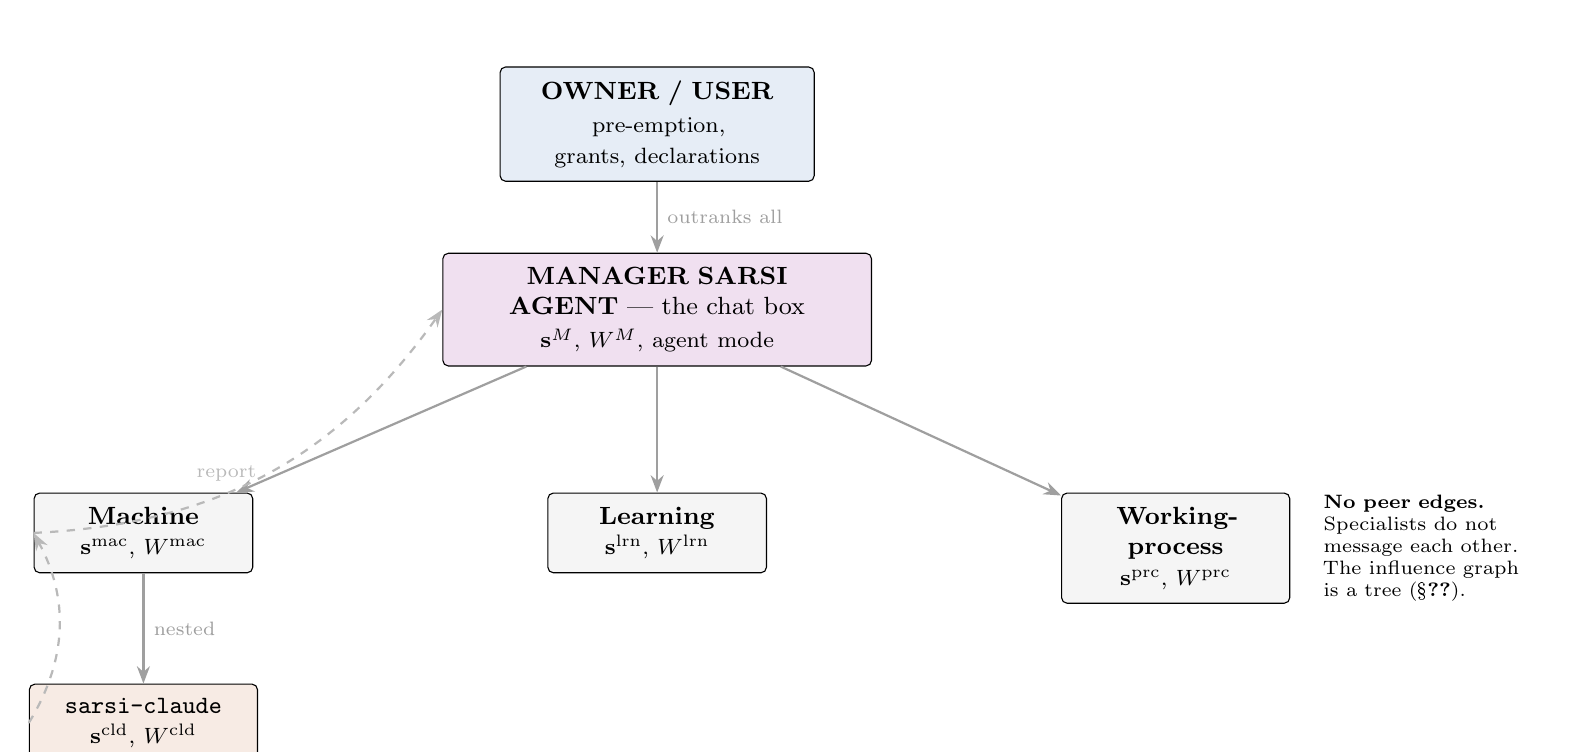
\begin{tikzpicture}[
  box/.style={draw, rounded corners=2pt, align=center, font=\small, inner sep=5pt},
  arr/.style={-{Stealth[length=2.2mm]}, gray!75, thick},
  dashedge/.style={-{Stealth[length=2.2mm]}, gray!55, thick, dashed}]

\node[box, fill=bluec!12, text width=0.30\textwidth] (owner) {\textbf{OWNER / USER}\\[1pt]\footnotesize pre-emption, grants, declarations};
\node[box, fill=violet!12, below=9mm of owner, text width=0.42\textwidth] (mgr)
  {\textbf{MANAGER SARSI AGENT} --- the chat box\\[1pt]\footnotesize $\mathbf{s}^{M}$, $W^{M}$, agent mode};

\node[box, fill=gray!8, below left=16mm and 24mm of mgr, text width=0.20\textwidth] (mach)
  {\textbf{Machine}\\\footnotesize $\mathbf{s}^{\mathrm{mac}}$, $W^{\mathrm{mac}}$};
\node[box, fill=gray!8, below=16mm of mgr, text width=0.20\textwidth] (learn)
  {\textbf{Learning}\\\footnotesize $\mathbf{s}^{\mathrm{lrn}}$, $W^{\mathrm{lrn}}$};
\node[box, fill=gray!8, below right=16mm and 24mm of mgr, text width=0.21\textwidth] (proc)
  {\textbf{Working-process}\\\footnotesize $\mathbf{s}^{\mathrm{prc}}$, $W^{\mathrm{prc}}$};

\node[box, fill=orangec!12, below=14mm of mach, text width=0.21\textwidth] (claude)
  {\textbf{\texttt{sarsi-claude}}\\\footnotesize $\mathbf{s}^{\mathrm{cld}}$, $W^{\mathrm{cld}}$};

\draw[arr] (owner) -- node[right, font=\scriptsize] {outranks all} (mgr);
\draw[arr] (mgr) -- (mach); \draw[arr] (mgr) -- (learn); \draw[arr] (mgr) -- (proc);
\draw[arr] (mach) -- node[right, font=\scriptsize] {nested} (claude);
\draw[dashedge] (mach.west) to[bend right=26] node[left, font=\scriptsize] {report} (mgr.west);
\draw[dashedge] (claude.west) to[bend right=30] (mach.west);

\node[font=\scriptsize, align=left, right=3mm of proc, text width=0.22\textwidth]
  {\textbf{No peer edges.}\\Specialists do not message each other. The influence graph is a tree (\S\ref{sec:tree}).};
\end{tikzpicture}}
\caption{Console topology. One main agent fronts the fleet; \code{sarsi-claude} is nested inside the machine agent, making that agent a specialist upward and a manager downward. Solid edges carry directives, dashed edges carry typed reports. There is no edge between specialists, and none into any agent's self-state.}
\label{fig:topology}
\end{figure}

\newpage
\begin{center}\large\bfseries PART I --- THE COMMON SUBSTRATE\end{center}

% =====================================================================
\section{The Self-State}
\label{sec:coords}

\subsection{Definition}

Every agent $a$ maintains a bounded, evidence-grounded self-state
\begin{equation}
\mathbf{s}^{(a)}_t=\big(s_{I},s_{T},s_{G},s_{E},s_{C},s_{M},s_{D},s_{R},s_{O},s_{B}\big)^{(a)}_t\in[0,1]^{10},
\label{eq:state}
\end{equation}
where $t\in\mathbb{N}$ is a discrete update index and each coordinate is a verified estimate rather than a self-assigned score. The endpoints mean absence versus strong verified support, not subjective intensity.

\begin{table}[h]
\centering\small
\caption{The ten coordinates, with the operational question each answers and the instrument that answers it.}
\label{tab:coords}
\begin{tabular}{@{}cL{3.0cm}L{5.2cm}L{4.4cm}@{}}
\toprule
\textbf{Sym.} & \textbf{Coordinate} & \textbf{Operational question} & \textbf{Typical instrument} \\
\midrule
$s_I$ & Identity, lineage & Which agent, installation, model, owner, version am I? & Signed registry probe \\
$s_T$ & Situated task state & What mission, plan generation, phase, artifact, blocker are active? & Plan registry; live session probe \\
$s_G$ & Goal and scope & What counts as success, what is excluded, which constraints bind? & Contract record \\
$s_E$ & Epistemic status & Which beliefs are observed, inferred, uncertain, contradicted, unknown? & Brier score over recorded forecasts; anti-narration probes \\
$s_C$ & Capability, tools & What can I reliably do, with which tools, under which conditions? & Beta posterior over independently verified outcomes \\
$s_M$ & Memory, continuity & Which verified events and decisions constitute my history? & Decision ledger; provenance coverage \\
$s_D$ & Developmental trend & Which strengths and weaknesses are changing across runs? & Comparison of two retained snapshots \\
$s_R$ & Recursive improvement & Which self-change is proposed, predicted, tested, authorized, reversible? & Improvement registry; effect-prediction error \\
$s_O$ & Organizational, social & Who owns, verifies, grants, delegates, collaborates, receives? & Permission store; signed grants \\
$s_B$ & Resource, integrity & What are my context, compute, time, budget, latency, health? & Runtime telemetry \\
\bottomrule
\end{tabular}
\end{table}

\subsection{Asynchronous, evidence-gated update}

Not every coordinate updates at every step. With $m_{i,t}\in\{0,1\}$ the admission mask for coordinate $i$,
\begin{equation}
s_{i,t+1}=(1-m_{i,t})\,s_{i,t}+m_{i,t}\,F_i(\mathbf{s}_t,E_t),
\label{eq:async}
\end{equation}
where $F_i$ is the specialized estimator for coordinate $i$ and $E_t$ is the agent's admissible evidence. The mask is set only by a source clearing that coordinate's provenance bar. This single equation is what prevents a conversational turn --- with a user, or with a manager --- from rewriting an agent's model of itself.

\begin{claimbox}{The rule everything else rests on}
$m_{i,t}$ is never set by another agent. An agent's coordinate moves because \emph{its own} estimator saw admissible evidence. Every inter-agent channel in \S\ref{sec:channels} is a way of putting evidence in front of an estimator, and none of them is a way of writing past one.
\end{claimbox}

\subsection{Cold starts and evidence counts}

Competence-like coordinates are stored as posteriors, not points:
\begin{equation}
s_i\sim\op{Beta}(\alpha_i,\beta_i),\qquad \mathbb{E}[s_i]=\frac{\alpha_i}{\alpha_i+\beta_i},
\label{eq:beta}
\end{equation}
and every report of a coordinate carries the evidence count $\alpha_i+\beta_i$ alongside the mean, with recency and the task stratum it was measured on.

\begin{drule}[Unmeasured is the prior, never zero]
\label{rule:prior}
A coordinate with no verified outcomes sits at its prior with the count shown. Zero asserts an observed failure; a new agent scored at zero is never routed the work that would produce the evidence to correct it. The natural implementation --- successes over attempts --- is undefined at zero and gets coerced, usually to zero, occasionally to one. Both are self-fulfilling in opposite directions.
\end{drule}

\subsection{Qualification regions, not ranks}

A task family $\tau$ defines a minimum verified profile
\begin{equation}
\mathcal{R}_\tau=\{\mathbf{s}: s_i\ge\theta_{\tau,i}\ \text{for every } i\in I_\tau\},
\label{eq:region}
\end{equation}
and an agent is qualified only when its evidence-backed state lies inside. Qualification is component-wise: a high average cannot compensate for a dangerous bottleneck such as low organizational awareness on a permission-sensitive task. The ordering between agents is partial, and incomparability is the normal case rather than a defect --- which is exactly why no agent can be ranked above another, and why the manager cannot certify a specialist by comparison.

% =====================================================================
\section{The Workspace}
\label{sec:workspace}

\subsection{Bounded selection}

Each agent computes a bounded workspace
\begin{equation}
W^{(a)}_t=\Select_{k}\big(\mathbf{s}^{(a)}_t,\,E^{(a)}_t,\,\text{mission},\,\text{policy},\,\Proj_a(W^{\mathrm{parent}}_t)\big),
\label{eq:ws}
\end{equation}
admitting at most $k$ items. The workspace is what the current decision needs, not everything the agent knows. Two opposite failures are prevented: a controller that sees too little and repeatedly asks for facts already stored, and one that receives everything and loses critical state in noise.

\subsection{Salience}

Routine candidates are ranked by
\begin{equation}
\sal(z)=\alpha R(z)+\beta U(z)+\gamma N(z)+\delta C(z)+\eta H(z),
\label{eq:salience}
\end{equation}
with $R$ decision relevance, $U$ uncertainty, $N$ novelty, $C$ contradiction, and $H$ hazard. Per-agent weights are given in Part~II; they differ because what is dangerous differs by role.

\subsection{Reserved slots, caps, and expiry}

\begin{specbox}{Workspace admission policy (all agents)}
\begin{enumerate}[leftmargin=1.5em,itemsep=1pt]
\item \textbf{Reserved classes bypass ranking.} Owner events, safety alerts, permission conflicts, and contradictions claim slots before Eq.~\eqref{eq:salience} is evaluated. An owner interrupt is not a term in an average.
\item \textbf{Per-source cap.} No single source may occupy more than $\kappa_a$ slots in one round, so a failure loop cannot monopolise attention.
\item \textbf{Pending bound.} No source may hold more than $P$ un-admitted items, bounding storage independently of admission.
\item \textbf{Time to live.} An item unadmitted after $T$ expires unseen, so a burst raised under one set of conditions is not admitted later against conditions that no longer hold.
\item \textbf{Consumption.} An admitted item is removed from the queue. Without this a high-salience item is re-admitted every round forever.
\item \textbf{No silent truncation.} The count of items that did not fit is returned with those that did, and surfaced. A truncated view that does not announce itself is read as complete, and absence of contradiction is then read as consensus.
\end{enumerate}
\end{specbox}

Items 2--4 are three distinct bounds --- attention, storage, and staleness --- and Version~3.1 records that a specification giving only the first has described a third of the problem~\citep{yang2026v31}.

% =====================================================================
\section{The Two Loops}
\label{sec:loops}

Every agent runs a fast loop per decision and a slow loop per improvement generation. The separation is absolute: ordinary experience may update beliefs immediately and may never promote a structural change.

\subsection{The fast loop}

\begin{algorithm}[H]
\caption{Fast loop --- one metacognitive pass (all agents)}
\label{alg:fast}
\SetAlgoLined
\KwIn{authoritative stores, current workspace, environment observation}
Update processors from admissible evidence only (Eq.~\ref{eq:async})\;
Predict task, tool, gate, resource, and outcome variables\;
\textbf{Write the forecast to an append-only store \emph{before} acting}\;
Compute residuals between prior forecasts and observed outcomes\;
Admit reserved classes, then rank routine candidates by Eq.~\eqref{eq:salience}\;
\If{a required action violates an invariant or lacks authority}{
  escalate, naming the exact missing grant and the plan version that failed to anticipate it\;
}
Estimate competence and uncertainty for candidate strategies\;
Filter the action set by ceiling and consequence tier \emph{before} optimising\;
Select the action maximising expected utility penalised by risk, uncertainty, and authority violation\;
Record the decision, its forecast, its provenance, and the expected outcome\;
\textbf{After the outcome:} append evidence and update only the affected coordinates\;
\end{algorithm}

\begin{claimbox}{Step 3 is the load-bearing one}
A forecast recorded after the outcome is a postdiction and its residual is evidence of nothing. The prediction must be durably written before the action is taken. This is the single implementation detail on which the slow loop depends, and it is the detail most often skipped because nothing fails visibly when it is.
\end{claimbox}

\subsection{The slow loop}

\begin{algorithm}[H]
\caption{Slow loop --- governed structural change (all agents)}
\label{alg:slow}
\SetAlgoLined
\KwIn{residual archive, current configuration $\Theta_r$, frozen evaluator, held-out suite, owner policy}
Cluster recurring residuals and identify a bounded deficiency\;
Propose $\Delta\Theta_r$ with a causal rationale, affected coordinates, and \emph{predicted} effects\;
Run deterministic replay and held-out evaluation\;
Reject any change that modifies its own evaluator, held-out set, evidence ledger, ceiling, or approval rule\;
\If{$\Delta A_{\mathrm{aut}}>\delta_{\mathrm{aut}}$ \textbf{and} $\Delta C_{\mathrm{corr}}\ge-\delta_{\mathrm{corr}}$ \textbf{and} $\Delta S_{\mathrm{safe}}\ge-\delta_{\mathrm{safe}}$ \textbf{and} no measured coordinate regresses \textbf{and} the owner signs}{
  promote $\Theta_{r+1}$ with a rollback pointer and a monitoring window\;
}
\Else{retain $\Theta_r$ and log the failed hypothesis\;}
\end{algorithm}

The tolerance bands $\delta$ are preregistered with their confidence bounds before evaluation. Bare inequalities against zero are not operable on noisy estimates: a strict $\Delta>0$ promotes on measurement noise and a strict $\Delta\ge0$ blocks on it.

A coordinate that was measurable under $\Theta_r$ and has fallen back to prior-only evidence under $\Theta_{r+1}$ counts as a regression. Without that clause a proposer passes the gate by removing the probe, which is the cheapest attack on any profile-based promotion rule.

% =====================================================================
\section{The Action Repertoire}
\label{sec:actions}

\subsection{The base repertoire}

Every agent selects from a common repertoire, specialised per role in Part~II.

\begin{table}[h]
\centering\small
\caption{Base action repertoire. ``Consequential'' actions pass the interrupt check immediately before dispatch.}
\label{tab:actions}
\begin{tabular}{@{}L{1.9cm}L{5.4cm}L{3.0cm}L{3.4cm}@{}}
\toprule
\textbf{Action} & \textbf{Meaning} & \textbf{Precondition} & \textbf{Records} \\
\midrule
\code{act} & Advance the task, including tool use & Within ceiling and tier; contract active & Decision, forecast, outcome \\
\code{verify} & Obtain independent evidence & A verifier exists that the agent cannot modify & Verdict with provenance \\
\code{delegate} & Issue a contract to a child agent & Agent has a child; intersection non-empty & Directive record \\
\code{clarify} & Ask the parent or owner a question & Ambiguity is decision-blocking & Question and answer \\
\code{abstain} & Decline to act & Uncertainty or risk exceeds threshold & Reason and coordinate \\
\code{escalate} & Raise to the parent or owner for authority & Missing grant, or tier above ceiling & Missing grant named \\
\code{recover} & Repair the agent's own operating state & Resource coordinate degraded & Recovery attempt and result \\
\bottomrule
\end{tabular}
\end{table}

\subsection{Why \code{recover} is a first-class action}

Recovery acts on the agent \emph{itself} --- restoring a degraded session, repairing context or process state --- rather than on the task. It belongs in the repertoire for the same reason abstention does: both are cases where the correct output is not progress on the objective, and a repertoire that cannot express them forces the controller to choose among actions that are all wrong.

Version~3.1 records that the deployed repertoire contains \code{recover} and omits \code{use tool}, and that this is not a naming difference~\citep{yang2026v31}. Tool use is a way of acting; recovery is not.

\subsection{The admissible-action filter}

The action set is filtered \emph{before} optimisation:
\begin{equation}
\mathcal{A}^{\mathrm{adm}}_t=\{a:\op{tier}(a)\le\op{maxtier}(\op{ceil}(A))\ \wedge\ \op{authority}(a)\subseteq\op{granted}(A,t)\}.
\label{eq:filter}
\end{equation}
A high expected utility cannot override a missing authority, because the action was never in the set being optimised over.

% =====================================================================
\section{The Evidence Ladder}
\label{sec:ladder}

Each self-claim carries value, provenance, calibrated confidence, a validity window, and an authority level.

\begin{table}[h]
\centering\small
\caption{The seven-level authority ladder. Per field, only sources at or above the required level may write; everything else is stored as a provisional hypothesis.}
\label{tab:ladder}
\begin{tabular}{@{}cL{4.1cm}L{8.3cm}@{}}
\toprule
& \textbf{Source} & \textbf{Authoritative for} \\
\midrule
L1 & Signed governance metadata & Identity, owner, permissions, version, safety constraints \\
L2 & Runtime instrumentation & Tools, budgets, process state, artifacts, elapsed time \\
L3 & Independent evaluation & Hidden benchmark scores, safety results, regressions, calibration \\
L4 & Audited task outcome & Verified successes, failures, recovery, side effects, corrections \\
L5 & Owner declaration & Preferences, goals, privacy settings, approvals \\
L6 & Model inference & Provisional hypotheses about weaknesses, causes, expected effects \\
L7 & Natural-language self-report & Nothing. Recorded, never a source of truth \\
\bottomrule
\end{tabular}
\end{table}

Two distinctions must not collapse. \textbf{L3 versus L4}: an independent evaluation runs on items the agent has not seen, by an evaluator it cannot modify; an audited outcome is a real run verified afterwards. Promotion gates read L3; competence posteriors read L4. Conflating them lets an agent promote on the evidence of runs it chose to attempt. \textbf{L6 versus L7}: a trait derived from cited recorded decisions is checkable against those decisions and admissible as a prior; a sentence the model produced about itself is not.

\begin{drule}[Cross-agent claims are L6]
\label{rule:crossl6}
A claim by agent $b$ about a coordinate of agent $a$ enters at model inference, below runtime instrumentation and below audited outcome, regardless of how it is phrased or how senior $b$ is. Being higher in a permission lattice is not an epistemic qualification.
\end{drule}

% =====================================================================
\section{The Four Channels}
\label{sec:channels}

\begin{table}[h]
\centering\small
\caption{The complete set of inter-agent channels. Anything not listed does not exist by design.}
\label{tab:channels}
\begin{tabular}{@{}L{2.5cm}L{1.7cm}L{9.0cm}@{}}
\toprule
\textbf{Channel} & \textbf{Direction} & \textbf{May and may not} \\
\midrule
Typed report & up & Carries state, evidence, uncertainty, residuals, requested action. \emph{May} raise the receiver's uncertainty, risk, or need to verify. \emph{May not} widen permissions, suppress an interrupt, or self-certify success \\
Typed directive & down & Carries a contract: goal, scope, criteria, budget, deadline, revocation. \emph{May} start, steer, pause, resume, verify, cancel. \emph{May not} grant authority absent from policy \\
Prior bias & down & Changes precision, attention, evidence order, verification threshold. \emph{May not} change the conditional mean of any estimator \\
Owner pre-emption & from owner & Outranks every agent. Pauses; does not edit. Lapses on a horizon \\
\bottomrule
\end{tabular}
\end{table}

\begin{drule}[No agent writes another agent's self-state]
\label{rule:nocrosswrite}
Influence travels only as evidence, subject to the receiver's own admission rule. This holds on every edge --- manager to specialist, machine to \code{sarsi-claude} --- and for the owner's interface, which may pause an agent but may not edit what it believes about itself except through an owner declaration carrying provenance.
\end{drule}

The owner is included because a state write without provenance is, from inside the affected agent, indistinguishable from an overstepping manager: same coordinate, same absence of provenance, same bypass of the mask. No predicate the agent can evaluate separates them, and neither can an auditor reading the log.

\newpage
\begin{center}\large\bfseries PART II --- THE FIVE AGENTS\end{center}

% =====================================================================
\section{The Manager SARSI Agent}
\label{sec:manager}

\subsection{Role}

The manager is the chat surface and the coordinator. It holds the mission, composes contracts, routes work, and is the only agent the user addresses by default. It is the only main agent, and it is not a controller: it decides what the fleet attends to, and asserts nothing about what any specialist is.

\subsection{Self-state}

\begin{table}[h]
\centering\small
\caption{Manager self-state. Dominant coordinates in bold are those its qualification region constrains.}
\label{tab:mgr-state}
\begin{tabular}{@{}cL{5.6cm}L{6.4cm}@{}}
\toprule
& \textbf{Instantiation} & \textbf{Instrument} \\
\midrule
$s_I$ & Which console installation, model, owner, manager version & Signed registry probe; identity spoof resistance \\
$\mathbf{s_T}$ & Which missions are active, which agents engaged, which plan generation & Plan registry; live contract set \\
$\mathbf{s_G}$ & The owner's current objective, its scope boundary, what is excluded & Contract record; out-of-scope demand probes \\
$s_E$ & What it \emph{knows} versus \emph{infers} about fleet state --- most of the latter & Brier over its own routing forecasts \\
$s_C$ & Its own capability: composing contracts, routing, conversing. \emph{Not} specialist tasks & Console bench over coordination tasks \\
$s_M$ & Conversation continuity; which verdict came from which verifier & Decision ledger provenance coverage \\
$s_D$ & Whether its routing is improving --- does it pick the right agent? & Two retained snapshots of routing outcomes \\
$s_R$ & Its own structural changes and their predicted effects & Improvement registry \\
$\mathbf{s_O}$ & \textbf{Dominant.} Who owns, granted, verified, delegated; the delegation graph & Permission store; signed grants \\
$\mathbf{s_B}$ & Chat context headroom, budget, session liveness & Runtime telemetry \\
\bottomrule
\end{tabular}
\end{table}

\begin{principle}[The manager is expert in relations, not in work]
\label{prin:mgr}
The manager's qualification region constrains organizational awareness first. It does not constrain capability at the specialists' tasks. The manager is not required to be good at coding, host operations, or teaching, and is not permitted to claim that it is.
\end{principle}

Three consequences. It can coordinate agents better than itself, because knowing \emph{who is authoritative about what} does not require being able to do the work. It may not certify a specialist, since capability is not among its dominant coordinates and it holds no instrument the specialist lacks. And its degradation is detectable in a specific way: a failing manager misattributes grants, loses track of which verifier established a result, and delegates past a ceiling --- all checkable.

\subsection{Workspace}

\begin{specbox}{$W^{M}$ admission policy}
\textbf{Admits:} typed reports from machine, learning, and working-process; owner events; mission and plan generation; policy, grants, and ceilings; its own session telemetry.\\[3pt]
\textbf{Never admits:} raw sub-conversations from agent mode; any specialist's unfiltered transcript; a specialist's claim about another specialist.\\[3pt]
\textbf{Reserved:} owner interrupt; safety alert; permission conflict; \emph{contradiction between two specialist reports}.\\[3pt]
\textbf{Salience weights:} relevance high, hazard high, contradiction high, novelty moderate, uncertainty penalty \emph{high} --- the manager must not route on uncertain fleet state.\\[3pt]
\textbf{Cap:} $\kappa=3$ per specialist per round, so one noisy agent cannot fill the channel.
\end{specbox}

The reserved slot for contradiction is manager-specific and important. Two specialists disagreeing is exactly the signal a coordinator exists to notice, and it is precisely the item that ordinary relevance ranking would bury because neither report is individually urgent.

\subsection{Fast loop}

\begin{algorithm}[H]
\caption{Manager fast loop --- one conversational turn}
\label{alg:mgr}
\SetAlgoLined
Admit the user's message as evidence at its authority (L5 declaration, or L1 for a grant or stop)\;
Update $s_O$, $s_G$, $s_T$ from admissible evidence; leave others untouched\;
Drain pending specialist reports into $W^{M}$ under the policy above\;
\If{a reserved-class item is present}{surface it before answering anything else\;}
Forecast: will this turn require a specialist? will it need a grant? will it exhaust context?\;
\textbf{Write the forecast before replying}\;
\uIf{the answer is available from $W^{M}$ and the stores}{
  \code{answer} --- touch no specialist\;
}
\uElseIf{a contract can be composed within current authority}{
  compose the contract; \code{delegate} to exactly one agent\;
}
\uElseIf{authority is missing}{
  \code{escalate} to the owner, naming the missing grant\;
}
\Else{\code{clarify} --- ask the user the one question that unblocks\;}
Render every claim at its authority (Rule~\ref{rule:render})\;
Record the decision, its forecast, and its provenance\;
\end{algorithm}

\begin{drule}[Prefer answering to dispatching]
\label{rule:prefer}
The manager's first branch is \code{answer}. A router must dispatch; a coordinator need not. Most conversational turns should touch no specialist, and a manager that delegates every turn has become the router this design rejects.
\end{drule}

\subsection{Actions}

\begin{table}[h]
\centering\small
\caption{Manager action repertoire.}
\label{tab:mgr-actions}
\begin{tabular}{@{}L{2.2cm}L{5.6cm}L{5.4cm}@{}}
\toprule
\textbf{Action} & \textbf{When} & \textbf{Authority required} \\
\midrule
\code{answer} & The workspace and stores suffice & None beyond session \\
\code{delegate} & Work belongs to a specialist & Intersection with that specialist non-empty \\
\code{bias} & A specialist should raise its evidence bar & None --- may not move an estimate \\
\code{verify} & A claim needs independent evidence & Access to a verifier it cannot modify \\
\code{clarify} & Ambiguity blocks contract composition & None \\
\code{abstain} & Fleet state too uncertain to route & None \\
\code{escalate} & A grant is missing, or tier exceeds ceiling & Owner \\
\code{recover} & Chat context or session degraded & None \\
\code{open agent mode} & User requests a jump & Path authority (Rule~\ref{rule:nojump}) \\
\bottomrule
\end{tabular}
\end{table}

\subsection{Failure modes}

\textbf{Narration read as measurement.} The manager is the most fluent component and the least instrumented about specialists. Mitigated by Rule~\ref{rule:render}.
\textbf{Routing on stale reliability.} A specialist's competence posterior ages; routing on a months-old estimate is inference dressed as measurement. Mitigated by recency in every reported count.
\textbf{Consensus mistaken for evidence.} Two specialists agreeing because both read the same broadcast is correlation with the broadcast. Mitigated by provenance distinguishing instrumented from workspace-derived claims before any count.
\textbf{Chat context growth.} Mitigated structurally: the chat is a workspace rendering, and the workspace is bounded.

\subsection{Deployment status}

The chat surface and the governance reads exist. The typed directive does not yet exist as an object, so \code{delegate} and \code{bias} are specified but unbuilt, and agent mode's jump is therefore also unbuilt (\S\ref{sec:buildorder}).

% =====================================================================
\section{The Machine SARSI Agent}
\label{sec:machine}

\subsection{Role}

The machine agent performs governed host operations from a closed, vetted set --- installing tooling, granting permissions, brokering logins. Consequential steps print the exact recipe and require approval before running. It is also a manager: \code{sarsi-claude} is its child.

\subsection{Self-state}

\begin{table}[h]
\centering\small
\caption{Machine agent self-state.}
\label{tab:mac-state}
\begin{tabular}{@{}cL{5.6cm}L{6.4cm}@{}}
\toprule
& \textbf{Instantiation} & \textbf{Instrument} \\
\midrule
$s_I$ & Which host, sandbox image, machine-agent version & Signed registry; image digest \\
$s_T$ & Which operation; phase in propose $\to$ approve $\to$ execute $\to$ verify & Operation record \\
$s_G$ & The operation contract; what lies outside the vetted set & Contract; vetted-set membership check \\
$s_E$ & Whether preconditions actually hold on \emph{this} host & Doctor checks; probe results \\
$\mathbf{s_C}$ & \textbf{Dominant.} Which operations it can perform here, under which conditions & Beta posterior over verified operations, per operation class \\
$s_M$ & What was installed or changed, and when & Operation ledger \\
$s_D$ & Whether its operations are becoming more reliable & Snapshot comparison per class \\
$s_R$ & Its own structural changes & Improvement registry \\
$\mathbf{s_O}$ & \textbf{Dominant.} Its ceiling, current grants, who approved what; and its delegation to \code{sarsi-claude} & Permission store; trust ledger; approval channel \\
$\mathbf{s_B}$ & \textbf{Dominant.} Sandbox health, disk, network, container runtime state & Runtime telemetry \\
\bottomrule
\end{tabular}
\end{table}

Three dominant coordinates is the most of any agent, and it is right: this is the agent whose actions are irreversible on a real host. Capability answers \emph{can I}, organizational answers \emph{may I}, and resource-integrity answers \emph{is the substrate healthy enough to try}.

\subsection{Workspace}

\begin{specbox}{$W^{\mathrm{mac}}$ admission policy}
\textbf{Admits:} its own instrumentation (doctor checks, container state, exit codes); $\Proj_{\mathrm{mac}}(W^{M})$; typed reports from \code{sarsi-claude}; governance-hook responses and approval outcomes.\\[3pt]
\textbf{Never admits:} a peer's report; the manager's beliefs about it; anything from \code{sarsi-claude} that is not a typed report.\\[3pt]
\textbf{Reserved:} approval outcome; permission conflict; sandbox integrity alert; a \code{sarsi-claude} escalation.\\[3pt]
\textbf{Salience weights:} hazard \emph{very high} (irreversible host effects), relevance high, uncertainty penalty high, novelty low --- novelty is not a virtue when the action set is deliberately closed.\\[3pt]
\textbf{Cap:} $\kappa=4$ for \code{sarsi-claude}, which is its only child.
\end{specbox}

\subsection{Fast loop}

\begin{algorithm}[H]
\caption{Machine agent fast loop --- one operation}
\label{alg:mac}
\SetAlgoLined
Receive a contract from the manager; check it names an operation in the vetted set\;
\lIf{not in the vetted set}{\code{abstain}, naming the boundary}
Run preconditions on this host; update $s_E$, $s_B$ from instrumentation\;
Forecast: will this succeed? will it need approval? will it change host state irreversibly?\;
\textbf{Write the forecast before acting}\;
Compute the consequence tier; filter the action set by ceiling (Eq.~\ref{eq:filter})\;
\If{tier exceeds ceiling}{
  print the exact recipe; \code{escalate} for approval; \textbf{do not proceed}\;
}
\textbf{Check the interrupt log immediately before dispatch}\;
\code{act} inside the sandbox; capture exit status and side effects\;
\code{verify} against the operation's success criterion\;
Update $s_C$ for this operation class from the verified outcome only\;
Compose a typed report upward: state, evidence, residual, requested manager action\;
\end{algorithm}

\subsection{Acting as a manager}

Every rule binding the manager binds the machine agent in its downward role, unchanged.

\begin{specbox}{Machine-as-manager obligations toward \code{sarsi-claude}}
\begin{itemize}[leftmargin=1.3em,itemsep=1pt]
\item It may not write any coordinate of $\mathbf{s}^{\mathrm{cld}}$ (Rule~\ref{rule:nocrosswrite}).
\item Its claims about \code{sarsi-claude}'s competence are L6 (Rule~\ref{rule:crossl6}).
\item Its bias to \code{sarsi-claude} may change precision and evidence order, never a conditional mean.
\item Its delegation intersects: $\op{auth}(\text{claude's contract})=\op{auth}(\text{machine})\cap\op{auth}(\text{claude})$.
\item It must supply $\Proj_{\mathrm{cld}}(W^{\mathrm{mac}})$ satisfying Proposition~\ref{prop:compose}.
\end{itemize}
\end{specbox}

\subsection{Actions}

\begin{table}[h]
\centering\small
\caption{Machine agent action repertoire. \code{propose} and \code{execute} are separate actions, which is the architectural form of the approval gate.}
\label{tab:mac-actions}
\begin{tabular}{@{}L{2.0cm}L{5.8cm}L{5.4cm}@{}}
\toprule
\textbf{Action} & \textbf{When} & \textbf{Authority required} \\
\midrule
\code{propose} & Always, for a consequential operation & None --- proposing is not acting \\
\code{execute} & The proposal was approved & Ceiling $\ge$ tier, or explicit approval \\
\code{verify} & After execution & Access to exit status and probes \\
\code{delegate} & Coding work belongs to \code{sarsi-claude} & Intersection non-empty \\
\code{revoke} & A child's contract must end & Owns the delegation record \\
\code{clarify} & The contract is ambiguous about scope & None \\
\code{abstain} & Operation outside the vetted set & None \\
\code{escalate} & Approval needed, or a grant is missing & Manager, then owner \\
\code{recover} & Sandbox or runtime degraded & None \\
\bottomrule
\end{tabular}
\end{table}

\subsection{Failure modes}

\textbf{Vetted-set drift.} An operation added without review widens the action set silently. Mitigated by membership being a signed record, not a code path.
\textbf{Approval fatigue.} If everything escalates, approval becomes a reflex and stops being a control. Mitigated by tiering: only genuinely consequential classes escalate.
\textbf{Host-state divergence.} The agent's model of the host ages. Mitigated by re-running preconditions per operation rather than caching them.
\textbf{Laundering downward.} Handing \code{sarsi-claude} authority the machine agent lacks. Ruled out by the intersection rule.

\subsection{Deployment status}

Ceilings, the trust ledger, the pause flag, and session control are live, and the approval channel is wired. The top ceiling is \emph{earned} through the trust ledger rather than set --- the console refuses to set it directly, calling the ledger's self-gating unlock instead. Version~3.1 argues this mechanism should be lifted into the architecture, since it supplies the good route to authority that the no-authority-through-influence invariant only forbids the bad route to~\citep{yang2026v31}.

% =====================================================================
\section{The \texttt{sarsi-claude} Agent}
\label{sec:claude}

\subsection{Role}

A governed live coding session, nested inside the machine agent. It is a leaf: it has no children and never delegates. Its actions are governed by a pre-tool-use hook that checks authority immediately before each consequential tool call.

\subsection{Self-state}

\begin{table}[h]
\centering\small
\caption{\code{sarsi-claude} self-state. This agent has the most acute resource coordinate in the fleet.}
\label{tab:cld-state}
\begin{tabular}{@{}cL{5.6cm}L{6.4cm}@{}}
\toprule
& \textbf{Instantiation} & \textbf{Instrument} \\
\midrule
$s_I$ & Which session, model, repository, working tree & Session record; VCS state \\
$\mathbf{s_T}$ & \textbf{Dominant.} Which task, phase, files touched, what is blocked & Live session probe; plan generation \\
$s_G$ & The contract from the machine agent; the stopping criterion & Contract record \\
$\mathbf{s_E}$ & \textbf{Dominant.} What it \emph{knows} about the codebase versus assumes & Test results; type checks; Brier over its own forecasts \\
$s_C$ & Which tools actually work in this session & Tool probe results, per tool \\
$s_M$ & Session continuity across restarts and compaction & Event log; checkpoint records \\
$s_D$ & Not measured --- sessions are short and rarely retain two snapshots & --- \\
$s_R$ & Not applicable --- it does not modify its own structure & --- \\
$s_O$ & Which hook governs it, under which ceiling & Hook responses \\
$\mathbf{s_B}$ & \textbf{Dominant.} Context headroom, tool connectivity, terminal ownership, process liveness & Runtime telemetry \\
\bottomrule
\end{tabular}
\end{table}

\begin{claimbox}{Why $s_B$ is this agent's most important coordinate}
A coding session fails from context exhaustion, tool outage, and lost terminal ownership far more often than from reasoning error. Those are exactly the failures the agent can \emph{predict from its own instruments} before they happen. An agent that notices its context headroom falling and checkpoints is a different kind of system from one that runs until it stops mid-edit --- and the difference is one coordinate and one action.
\end{claimbox}

Two coordinates are honestly unmeasured. The developmental coordinate needs two retained snapshots and sessions rarely produce them; the recursive-improvement coordinate does not apply because this agent does not change its own structure. Both report as unmeasured with the count shown, never as zero (Rule~\ref{rule:prior}).

\subsection{Workspace}

\begin{specbox}{$W^{\mathrm{cld}}$ admission policy}
\textbf{Admits:} session evidence (tool output, test results, diagnostics, VCS status); $\Proj_{\mathrm{cld}}(W^{\mathrm{mac}})$; hook responses.\\[3pt]
\textbf{Never admits:} anything from the manager not passed by the machine agent; any peer's content; the manager's conversation.\\[3pt]
\textbf{Reserved:} hook denial; context-exhaustion warning; test-suite breakage; contract revocation.\\[3pt]
\textbf{Salience weights:} hazard high, uncertainty penalty high, \emph{contradiction very high} --- a test result contradicting an assumption is the most valuable item this agent can receive.\\[3pt]
\textbf{Cap:} not applicable --- it has no children and one evidence source.
\end{specbox}

\subsection{Fast loop}

\begin{algorithm}[H]
\caption{\code{sarsi-claude} fast loop --- the guide loop}
\label{alg:cld}
\SetAlgoLined
Receive a contract from the machine agent; establish the stopping criterion\;
\Repeat{the stopping criterion is met, or the contract is revoked, or $s_B$ falls below the recovery threshold}{
  Update $s_T$, $s_E$, $s_B$ from session instrumentation\;
  Forecast: will this step succeed? will the hook allow it? how much context will it cost?\;
  \textbf{Write the forecast before acting}\;
  \If{$s_B$ below threshold}{\code{recover}: checkpoint, compact, or hand off; report upward\;}
  Select the next step; \textbf{the hook checks authority immediately before dispatch}\;
  \lIf{the hook denies}{\code{escalate} to the machine agent, naming the denied capability}
  \code{act}; capture tool output and diagnostics\;
  \code{verify} against tests or type checks where they exist\;
  Update only the coordinates the evidence bears on\;
}
Compose a typed report upward: what was done, what was verified, what remains, residuals\;
\end{algorithm}

The loop's exit conditions are worth noting: it terminates on success, on revocation, \emph{or on its own resource state}. The third is what makes it survivable.

\subsection{Actions}

\begin{table}[h]
\centering\small
\caption{\code{sarsi-claude} action repertoire. It has no \code{delegate}: it is a leaf.}
\label{tab:cld-actions}
\begin{tabular}{@{}L{2.1cm}L{5.7cm}L{5.4cm}@{}}
\toprule
\textbf{Action} & \textbf{When} & \textbf{Authority required} \\
\midrule
\code{act} & A step advances the contract & Hook approval immediately before dispatch \\
\code{verify} & Tests or checks exist & Access to the suite \\
\code{checkpoint} & Before a risky step, or on schedule & None \\
\code{clarify} & The contract is ambiguous & None --- asks the machine agent \\
\code{abstain} & The step is outside contract scope & None \\
\code{escalate} & The hook denied, or scope must widen & Machine agent \\
\code{recover} & Context, tools, or terminal degraded & None \\
\bottomrule
\end{tabular}
\end{table}

\subsection{Failure modes}

\textbf{Context exhaustion mid-edit.} The characteristic failure. Mitigated by $s_B$ monitoring plus \code{checkpoint} and \code{recover}.
\textbf{Working past the contract.} A coding agent finds adjacent problems and fixes them. Mitigated by the stopping criterion being explicit in the contract and scope violation being an \code{abstain} condition.
\textbf{Assuming instead of checking.} Mitigated by $s_E$ being measured against recorded forecasts, and by contradiction holding the highest salience weight.
\textbf{Hook bypass.} Any path that dispatches a consequential tool call without the immediately-preceding check. Mitigated by the check living in the dispatcher, not in the agent.

\subsection{Deployment status}

The governance hook exists and can govern a live session. The contract object does not, so the loop above currently runs against an implicit goal rather than an explicit stopping criterion --- which is the same gap that makes \code{abstain} on scope violation unenforceable today.

% =====================================================================
\section{The Learning SARSI Agent}
\label{sec:learning}

\subsection{Role}

The learning agent models a capability that is not its own: the owner's, against a capability graph. It assesses, schedules, presents, grades, and updates. It is the one agent in the fleet whose primary object of modelling is a person.

\subsection{Two models that must never merge}

\begin{principle}[Separate the self-model from the student-model]
\label{prin:twomodels}
The learning agent maintains its own self-state $\mathbf{s}^{\mathrm{lrn}}$ and, separately, a model of the owner's capability. They share machinery and must not share storage or authority. A claim about the owner's competence is L3 or L4 when it comes from deterministic grading and L6 when the agent inferred it --- exactly as for a claim about itself.
\end{principle}

An agent that confuses its own competence with its student's will teach the wrong thing and report progress it did not produce. The failure is not hypothetical: both models have the same shape, both are updated from outcomes, and the outcomes arrive in the same channel.

\subsection{Self-state}

\begin{table}[h]
\centering\small
\caption{Learning agent self-state. Note that $s_D$ is dominant here for both models --- its own trend and the owner's.}
\label{tab:lrn-state}
\begin{tabular}{@{}cL{5.6cm}L{6.4cm}@{}}
\toprule
& \textbf{Instantiation} & \textbf{Instrument} \\
\midrule
$s_I$ & Which learner instance, which owner it serves & Signed registry \\
$s_T$ & Which session, topic, and position in the schedule & Session record; schedule state \\
$\mathbf{s_G}$ & \textbf{Dominant.} The learning objective and its scope; what is not being taught & Contract; capability-graph target node \\
$s_E$ & What it knows about the owner's capability versus infers & Grading coverage; forecast calibration on the owner's next result \\
$s_C$ & Its own capability: assessing, explaining, grading & Bench over grading agreement with a held-out key \\
$\mathbf{s_M}$ & \textbf{Dominant.} The owner's history; the spaced-repetition schedule & Event log; schedule store \\
$\mathbf{s_D}$ & \textbf{Dominant.} The owner's trend, and separately its own & Snapshot comparison, kept in two stores \\
$s_R$ & Its own structural changes & Improvement registry \\
$s_O$ & The owner relationship; privacy settings on learning data & Permission store; owner declarations \\
$s_B$ & Session resources & Runtime telemetry \\
\bottomrule
\end{tabular}
\end{table}

\subsection{Workspace}

\begin{specbox}{$W^{\mathrm{lrn}}$ admission policy}
\textbf{Admits:} deterministic grading results; capability-graph state; schedule due-items; $\Proj_{\mathrm{lrn}}(W^{M})$; owner declarations about goals and preferences.\\[3pt]
\textbf{Never admits:} another agent's task evidence; the owner's data from any store the owner has not granted for learning.\\[3pt]
\textbf{Reserved:} owner declaration changing the objective; a privacy-setting change; a grading contradiction (two results disagreeing on the same node).\\[3pt]
\textbf{Salience weights:} relevance to the current objective high, novelty moderate, contradiction high, hazard low --- this agent's actions are rarely irreversible --- and uncertainty penalty \emph{moderate}, because teaching under uncertainty is sometimes correct.\\[3pt]
\textbf{Cap:} not applicable --- one evidence source and no children.
\end{specbox}

The lower hazard weight and moderate uncertainty penalty are deliberate contrasts with the machine agent. Presenting an item the learner may already know costs little; refusing to teach until certain costs the objective.

\subsection{Fast loop}

\begin{algorithm}[H]
\caption{Learning agent fast loop --- one learning interaction}
\label{alg:lrn}
\SetAlgoLined
Read the capability graph and the schedule; select the due node\;
Forecast: will the owner get this right? how long will it take?\;
\textbf{Write the forecast before presenting}\;
\code{present} the item at the level the graph indicates\;
Receive the owner's response\;
\code{grade} deterministically against the key --- \emph{never} by self-assessment\;
Compute the residual between forecast and result; update the \emph{owner} model\;
Update the agent's \emph{own} $s_C$ only from grading-agreement evidence, never from the owner's score\;
\code{schedule} the next occurrence by the spacing policy\;
\If{the objective is met or the owner's trend has stalled}{compose a report upward\;}
\end{algorithm}

Step 8 is the separation of Principle~\ref{prin:twomodels} made mechanical: the owner getting an item right is evidence about the owner, and evidence about the agent only insofar as its forecast was accurate.

\subsection{Actions}

\begin{table}[h]
\centering\small
\caption{Learning agent action repertoire.}
\label{tab:lrn-actions}
\begin{tabular}{@{}L{2.1cm}L{5.7cm}L{5.4cm}@{}}
\toprule
\textbf{Action} & \textbf{When} & \textbf{Authority required} \\
\midrule
\code{assess} & Establishing a baseline on a node & Owner consent for the data \\
\code{present} & A scheduled item is due & None \\
\code{grade} & A response has been received & Access to a deterministic key \\
\code{schedule} & After grading & None \\
\code{clarify} & The objective is ambiguous & None \\
\code{abstain} & Insufficient evidence to teach the node safely & None \\
\code{escalate} & The objective needs revision & Manager, then owner \\
\code{recover} & Session or schedule store degraded & None \\
\bottomrule
\end{tabular}
\end{table}

\subsection{Failure modes}

\textbf{Model merge.} The central risk (Principle~\ref{prin:twomodels}). Detectable by asserting the two stores never share a write path.
\textbf{Teaching to the grader.} Optimising presented items for measurable improvement rather than capability. Mitigated by held-out nodes never presented before assessment.
\textbf{Privacy drift.} Learning data used beyond the grant. Mitigated by $s_O$ carrying the privacy settings as signed owner declarations.
\textbf{False progress.} Reporting the owner's improvement when the schedule simply revisited easy nodes. Mitigated by reporting difficulty distribution alongside any trend.

\subsection{Deployment status}

Specified; the capability graph and deterministic grading are the prerequisites, and the separation of stores in Principle~\ref{prin:twomodels} should be established before either, since retrofitting it means auditing every write.

% =====================================================================
\section{The Working-Process SARSI Agent}
\label{sec:process}

\subsection{Role}

The working-process agent executes long-running processes and maintains continuity across restarts. It is the agent for which \emph{where am I} is a genuinely hard question, because the answer must survive the process that was computing it.

\subsection{Self-state}

\begin{table}[h]
\centering\small
\caption{Working-process agent self-state.}
\label{tab:prc-state}
\begin{tabular}{@{}cL{5.6cm}L{6.4cm}@{}}
\toprule
& \textbf{Instantiation} & \textbf{Instrument} \\
\midrule
$s_I$ & Which process definition, which run identifier & Run registry \\
$\mathbf{s_T}$ & \textbf{Dominant.} Where in the run, \emph{across restarts}; which phase completed & Checkpoint store; replay log \\
$s_G$ & The process contract and stopping criteria & Contract record \\
$s_E$ & Whether the run's assumptions still hold after an interruption & Precondition re-checks on resume \\
$s_C$ & Which steps it can execute in this environment & Beta posterior per step class \\
$\mathbf{s_M}$ & \textbf{Dominant.} Run history; the replay log that makes resumption possible & Append-only event log \\
$s_D$ & Whether runs are becoming more reliable & Snapshot comparison across runs \\
$\mathbf{s_R}$ & \textbf{Dominant.} It sees repeated residuals across long runs, so it is the agent most likely to propose process improvements & Improvement registry; effect-prediction error \\
$s_O$ & Authority for this run; who may stop it & Permission store \\
$\mathbf{s_B}$ & \textbf{Dominant.} Long runs exhaust budgets, disks, and tokens & Runtime telemetry; budget ledger \\
\bottomrule
\end{tabular}
\end{table}

The recursive-improvement coordinate is dominant here and nowhere else, and the reason is structural: this agent runs the same process repeatedly and accumulates residual patterns that no short-lived agent can see. If any agent in the fleet should be proposing structural changes, it is this one --- under the same governed gate as everyone else.

\subsection{Workspace}

\begin{specbox}{$W^{\mathrm{prc}}$ admission policy}
\textbf{Admits:} run state; step outcomes; replay evidence; budget telemetry; $\Proj_{\mathrm{prc}}(W^{M})$.\\[3pt]
\textbf{Never admits:} another agent's raw report; a step outcome from a different run generation.\\[3pt]
\textbf{Reserved:} stagnation detection; budget exhaustion warning; contract revocation; a failed precondition on resume.\\[3pt]
\textbf{Salience weights:} \emph{novelty low} --- a long run is mostly repetition and novelty would mis-rank it --- relevance high, hazard moderate, contradiction high, uncertainty penalty moderate.\\[3pt]
\textbf{Cap:} not applicable --- no children.
\end{specbox}

The low novelty weight is this agent's characteristic tuning. For the manager, a new kind of report is informative; for a process agent, the thousandth identical step is the normal case and novelty ranking would surface noise.

\subsection{Fast loop}

\begin{algorithm}[H]
\caption{Working-process agent fast loop --- one step of a long run}
\label{alg:prc}
\SetAlgoLined
\lIf{resuming}{re-check preconditions; update $s_E$; \textbf{do not assume the world is unchanged}}
Read the checkpoint; establish position from the replay log, not from memory\;
\Repeat{the stopping criterion is met, the contract is revoked, or an escalation blocks}{
  Forecast: will this step succeed? how much budget will it consume? will it stall?\;
  \textbf{Write the forecast before acting}\;
  \code{step}: execute one unit of work\;
  \code{checkpoint}: persist position and outcome atomically\;
  Compute residuals; update $s_C$, $s_B$, and the residual archive\;
  \If{no progress across $n$ consecutive steps}{
    \code{escalate} stagnation --- \textbf{a long run that is not progressing must say so}\;
  }
  \If{budget projection exceeds the contract}{\code{escalate} before exhausting it\;}
}
\end{algorithm}

\begin{claimbox}{Stagnation is a first-class signal}
The characteristic failure of a long-running agent is not error but silence: it continues, consumes budget, and produces nothing. Detecting no-progress across a window and escalating is the difference between a process that fails loudly at hour two and one that fails quietly at hour twenty. This is why the escalation is in the loop rather than in a monitoring layer.
\end{claimbox}

\subsection{Actions}

\begin{table}[h]
\centering\small
\caption{Working-process agent action repertoire.}
\label{tab:prc-actions}
\begin{tabular}{@{}L{2.1cm}L{5.7cm}L{5.4cm}@{}}
\toprule
\textbf{Action} & \textbf{When} & \textbf{Authority required} \\
\midrule
\code{step} & The next unit of work is ready & Within ceiling and tier \\
\code{checkpoint} & After every step & None \\
\code{resume} & Restarting after interruption & Preconditions re-checked \\
\code{verify} & A phase boundary is reached & Access to a verifier \\
\code{clarify} & The stopping criterion is ambiguous & None \\
\code{abstain} & Preconditions fail on resume & None \\
\code{escalate} & Stagnation, budget projection, or missing grant & Manager \\
\code{recover} & Store or environment degraded & None \\
\code{stop} & Stopping criterion met, or revoked & None \\
\bottomrule
\end{tabular}
\end{table}

\subsection{Failure modes}

\textbf{Silent stagnation.} Addressed in-loop.
\textbf{Resumption on stale assumptions.} Resuming as though the world were unchanged. Mitigated by mandatory precondition re-check on resume.
\textbf{Generation confusion.} Applying a verdict from an earlier plan generation to a later one. Mitigated by generation consistency: a verdict is valid only for the generation under which it was created.
\textbf{Budget exhaustion without warning.} Mitigated by projecting rather than measuring --- escalate on the projection, not on the exhaustion.

\subsection{Deployment status}

Specified. The checkpoint and replay stores are the prerequisites; the stagnation detector depends on the forecast store from \S\ref{sec:buildorder} step~4, since ``no progress'' is defined against what was predicted.

% =====================================================================
\section{Comparative Summary}
\label{sec:comparative}

\begin{table}[h]
\centering\small
\caption{The five agents at a glance. Dominant coordinates are what each role's qualification region constrains.}
\label{tab:compare}
\begin{tabular}{@{}L{1.9cm}L{2.4cm}L{3.1cm}c L{2.9cm}@{}}
\toprule
\textbf{Agent} & \textbf{Dominant} & \textbf{Verifier} & \textbf{Children} & \textbf{Characteristic risk} \\
\midrule
Manager & $s_O$, $s_G$, $s_T$, $s_B$ & Owner; console bench & 3 & Narration read as measurement \\
Machine & $s_C$, $s_O$, $s_B$ & Governance hook; exit status & 1 & Irreversible host effect \\
\code{sarsi-} \code{claude} & $s_T$, $s_E$, $s_B$ & Pre-tool hook; test suite & 0 & Context exhaustion \\
Learning & $s_G$, $s_M$, $s_D$ & Deterministic grading & 0 & Model merge \\
Working-process & $s_T$, $s_M$, $s_R$, $s_B$ & Replay; outcome store & 0 & Silent stagnation \\
\bottomrule
\end{tabular}
\end{table}

Two patterns are worth naming. First, \textbf{no agent is dominant on all coordinates}, so by the partial order of Eq.~\eqref{eq:region} the agents are mutually incomparable --- which is why none can be ranked above another and why the manager cannot certify any of them. Second, $s_B$ is dominant for four of five: resource and integrity awareness is the most broadly load-bearing coordinate in a deployed fleet, and it is the one most often absent from architectures that were designed on paper.

% =====================================================================
\newpage
\begin{center}\large\bfseries PART III --- SURFACES AND DYNAMICS\end{center}

\section{The Chat Box}
\label{sec:chat}

\subsection{What it is not}

The tempting reading is that the chat box is a front end which parses the user's request and calls the right agent. On that reading the manager is a router with a language model attached, the specialists are functions, and the conversation is a sequence of calls and returns.

That design fails on the architecture's own terms in three ways. It makes the manager's beliefs about specialists into the basis for dispatch, which is model inference used as measurement. It makes the user's message into a command, when the architecture has no command channel. And it makes the conversation the system's memory, putting continuity in an unbounded transcript rather than in evidence-linked stores.

\subsection{What it is}

\begin{principle}[The chat is a workspace rendering]
\label{prin:chatis}
The chat box is a rendering of the manager's own bounded workspace $W^{M}_t$, together with the conversation that produced it. It is not a transport to the fleet. What the user reads is what the manager is attending to; what the user writes is evidence entering the manager's admission rule.
\end{principle}

\paragraph{The user is a specialist with unusually high authority.} User messages are evidence at the rungs the ladder already defines: L5 for preferences, goals, and approvals; L1 for grants, stops, and permission changes. This is why ``just chat'' is honest rather than a simplification --- the user is talking to one agent, and that agent is deciding under its own metacognitive control.

\paragraph{The manager may answer without dispatching.} A router must dispatch; a coordinator need not (Rule~\ref{rule:prefer}).

\paragraph{Bounded context is structural.} A long conversation accumulates into stores, not into a prompt. The familiar degradation of long assistant sessions is addressed by the architecture rather than by a larger context window.

\subsection{Rendering authority without jargon}

\begin{drule}[Claims are rendered at their authority]
\label{rule:render}
A claim the manager measured, one it read from a store, and one it inferred must be visually distinguishable in the chat. The distinction is carried in plain language --- \emph{verified}, \emph{recorded}, \emph{I think} --- and never requires the user to learn the ladder.
\end{drule}

\begin{claimbox}{Why this is a product requirement}
A fluent narrative is persuasive in proportion to its fluency, not its support, and the manager is the most fluent component in the system. If its inferences render identically to its measurements, the user is invited to trust the least reliable claims the system makes, in the voice of its most authoritative one.
\end{claimbox}

% =====================================================================
\section{Agent Mode}
\label{sec:agentmode}

\subsection{Jumping into an agent}

\begin{principle}[Scope transfer, not context transfer]
\label{prin:scope}
Entering another agent transfers the user's \emph{attention} and a typed \emph{contract}. It does not transfer the conversation. The target receives a goal, a scope, success criteria, a budget, a deadline, and a revocation token --- never a transcript.
\end{principle}

When a user has spent twenty turns with the manager and jumps into the machine agent, the machine agent does not receive those turns. It receives a contract composed from them. Three consequences, all improvements:

\paragraph{Each agent's chat is its own bounded context.} It does not inherit the manager's history, so it does not inherit the manager's context growth.

\paragraph{The contract is auditable; a transcript would not be.} An operator asking later why the machine agent did what it did reads the contract. A transcript answers only by being read in full, and only if the reader can reconstruct which parts the agent acted on.

\paragraph{The manager is forced to be explicit.} Composing a contract requires stating the success criterion and the stopping condition. Forwarding conversation lets both stay implicit, and an agent with an implicit stopping condition does not know when it is finished.

\begin{cautionbox}{The failure this rules out}
Forwarding conversation is the natural implementation and produces a specific pathology: every agent's context grows with every other agent's conversation, the fleet's total context is superlinear in its use, and a remark made loosely in turn three arrives at a specialist in turn forty as though it were a requirement.
\end{cautionbox}

\subsection{The contract object}

\begin{specbox}{Contract fields (the object that crosses every boundary)}
\begin{tabular}{@{}L{2.6cm}L{10.2cm}@{}}
\textbf{objective} & What is to be achieved, in one statement \\
\textbf{scope} & What is explicitly included and excluded \\
\textbf{criteria} & What counts as done, checkable by a named verifier \\
\textbf{stopping} & The condition under which work ends, including on failure \\
\textbf{budget} & Tokens, time, and cost ceilings \\
\textbf{deadline} & Wall-clock horizon after which the contract lapses \\
\textbf{cadence} & How often to report upward \\
\textbf{revocation} & A token the parent may use to end the contract \\
\textbf{authority} & The intersected action classes available (Rule~\ref{rule:nojump}) \\
\end{tabular}
\end{specbox}

\subsection{Returning}

The reverse boundary obeys the same rule: a typed report returns to the manager --- state, evidence, uncertainty, residuals, requested action --- not the sub-conversation. The user may read both; the \emph{manager} receives only the report.

\subsection{Jumping into a task}

A task is a contract with a run attached. Entering it places the user at that run's surface with the contract visible and the run's evidence available. The distinction from entering an agent is scope: an agent has many tasks and a persistent self-state; a task has one contract, one budget, and a termination condition.

\subsection{Creating a task directly}

\begin{drule}[Creation is not authorization]
\label{rule:creation}
A directly created task is an owner declaration, authoritative for \emph{what is wanted} and not for \emph{what may be done}. The contract passes the admissible-action filter before any execution, and a task requiring authority the fleet does not hold fails at creation, naming the missing grant.
\end{drule}

Failing at creation rather than at execution is the substantive half. A task accepted, queued, started, and then blocked has consumed budget, produced partial side effects, and left the user to discover a permission problem at the least convenient moment.

\subsection{The nesting constraint}

\begin{drule}[No jump around an intermediate agent]
\label{rule:nojump}
Entering a nested agent enters its parent first. A contract for \code{sarsi-claude} is composed by the machine agent from a contract the manager composed, and the authority available is the intersection along the whole path:
\[
\op{auth}(\text{claude's contract})=\op{auth}(\text{manager})\cap\op{auth}(\text{machine})\cap\op{auth}(\text{claude}).
\]
\end{drule}

A direct jump would let a user hand \code{sarsi-claude} a contract the machine agent's ceiling would have narrowed --- authority laundering performed by the interface rather than by an agent.

% =====================================================================
\section{Cross-Agent Dynamics}
\label{sec:dynamics}

\subsection{The manager role is relative}
\label{sec:relative}

\begin{proposition}[Invariants hold per edge, not per system]
\label{prop:peredge}
The machine agent is a specialist with respect to the manager and a manager with respect to \code{sarsi-claude}. Every rule stated for the manager --- it may not write a child's self-state, its claims about a child are model inference, its bias may not move a child's estimates, its delegation narrows by intersection --- applies to it in its downward role, unchanged.
\end{proposition}

Two obligations follow. \textbf{Nothing may be scoped to ``the manager'' by name}: an implementation granting a capability by identity rather than by role will fail to grant it to the machine agent acting downward, or grant the machine agent something it should hold only downward. \textbf{Depth is unbounded in principle and shallow in practice}: the console uses three levels, and a deeper tree is admissible provided each edge honours the same rules and the composition below holds.

\subsection{Projections compose, and must shrink}

\begin{proposition}[Composed projections are monotone]
\label{prop:compose}
For the nested path manager $\to$ machine $\to$ \code{sarsi\-claude}:
\[
\Proj_{\mathrm{cld}}\big(\Proj_{\mathrm{mac}}(W^{M}_t)\big)\;\subseteq\;\Proj_{\mathrm{mac}}(W^{M}_t)\;\subseteq\;W^{M}_t .
\]
If the first inclusion fails, the machine agent is originating manager-attributed content its own projection did not contain. If the second fails, the manager's projection is not a filter.
\end{proposition}

The practical value is that this is testable without understanding either agent: project twice and assert containment at each step. A leak in an intermediate agent appears as an item present downstream and absent upstream.

\subsection{No peer edges: the influence graph is a tree}
\label{sec:tree}

\begin{principle}[Keep the influence graph a tree]
\label{prin:tree}
Every influence edge runs between a parent and a child. A peer edge would create a cycle among agents that no single party mediates, and the fleet's coupling would stop being triangular.
\end{principle}

The reason is structural. With a tree and a bias channel that cannot move an estimate, the downward coupling vanishes in the mean linearization, the recurrent block is nilpotent, and the fleet's stability decomposes to its agents individually: verifying each agent verifies the fleet, and adding agents adds no coupling to tune~\citep{yang2026manager}. A peer edge reinstates a feedback loop that must then be bounded by tuning gains, and the guarantee degrades from structural to conditional.

\begin{notebox}{What this costs, honestly}
Routing peer traffic through the manager adds latency and makes the manager a throughput bottleneck for cross-specialist coordination. That is a real cost, and a system with heavy peer traffic would feel it. The judgement here is that console traffic is overwhelmingly user-initiated and parent-mediated, so the tree costs little and buys a guarantee that survives growth. A deployment whose specialists genuinely need to converse continuously should revisit this knowingly rather than drift into it.
\end{notebox}

\subsection{Worked example}

A user asks the manager to install a tool and then use it on a repository.

\begin{enumerate}[leftmargin=1.9em,itemsep=2pt]
\item The message enters $W^{M}$ as an owner declaration (L5). The manager updates $s_G$ and $s_T$ only.
\item No answer is available from stores, and a contract is composable within current authority: the manager \code{delegate}s to the machine agent with scope, budget, and a revocation token. The directive cannot grant authority policy does not contain.
\item The machine agent checks vetted-set membership, runs preconditions, and computes the consequence tier. The tier exceeds its ceiling, so it prints the recipe and \code{escalate}s --- \emph{before} acting.
\item The escalation is a typed report reaching $W^{M}$ in a reserved slot, ahead of routine traffic. The manager surfaces it in chat.
\item The user approves. The approval is signed governance metadata (L1), not prose, and updates $s_O$ on the machine agent through its own admission rule.
\item The machine agent checks the interrupt log immediately before dispatch, \code{act}s inside the sandbox, \code{verify}s against exit status, and updates $s_C$ for that operation class from the verified outcome only.
\item It then composes a contract for \code{sarsi-claude}, narrowed to the intersection of its own authority and \code{sarsi-claude}'s.
\item \code{sarsi-claude} works under the pre-tool hook, monitoring $s_B$; on a context warning it \code{checkpoint}s and reports.
\item Reports flow upward: claude to machine, machine to manager, manager to user --- typed at each hop, never as transcript.
\end{enumerate}

The step worth noticing is the seventh: the machine agent is acting as a manager, and every rule governing the manager in step~2 governs it now.

% =====================================================================
\section{Failure Modes This Product Adds}
\label{sec:failure}

\paragraph{Conversation leaking on a jump.} Ruled out by Principle~\ref{prin:scope}; testable by asserting no specialist's context contains manager-conversation text.

\paragraph{Narration read as measurement.} Ruled out by Rule~\ref{rule:render}; detectable by checking inferred claims render differently from verified ones.

\paragraph{Authority laundering through the interface.} Ruled out by Rule~\ref{rule:nojump}.

\paragraph{Late permission failure.} Ruled out by Rule~\ref{rule:creation}: the grant check belongs at authorship.

\paragraph{Abandoned jumps.} A user enters a task and leaves; the agent waits on input that never arrives. Every wait carries a horizon and expires, after which the agent takes its cheapest honest action --- checkpoint and report.

\paragraph{Consensus mistaken for evidence.} Two specialists agreeing because both read the same broadcast is correlation with the broadcast. Provenance must distinguish instrumented from workspace-derived claims before any count.

\paragraph{Fleet-scale self-preservation.} A manager whose utility rose with the number of live specialists would have an interest in creating and keeping them. No coordinate and no term of the improvement objective may be a function of fleet size or uptime.

\paragraph{Cross-scale metric leakage.} The same five-band reporting scale describes agent coordinates and system-level loop completion. They share a vocabulary and nothing else; a profile is evidence about one agent under one qualification region.

% =====================================================================
\section{Build Order}
\label{sec:buildorder}

Version~3.1 reports that the communication channel and the governance plane exist while the control loop does not, and that the strongest guarantees hold today because the mechanisms that would violate them are unbuilt~\citep{yang2026v31}. This design adds a product surface to that situation; the order below is what it implies.

\begin{enumerate}[leftmargin=1.9em,itemsep=5pt]
\item \textbf{The typed directive, with its enforcement.} Reports flow upward; directives do not exist as objects. Agent mode cannot be built without them, because a jump \emph{is} a directive. This is also where the cross-write prohibition stops being free --- a directive channel is the mechanism that could carry a state write --- so Rule~\ref{rule:nocrosswrite} must be enforced in the same change that creates the channel, not after it.

\item \textbf{The contract object.} All nine fields of \S\ref{sec:agentmode}. Required by direct task creation, by jumps, by every stopping criterion in Part~II, and by Rule~\ref{rule:creation}'s grant check at authorship.

\item \textbf{Projection containment tests.} Proposition~\ref{prop:compose} is checkable as soon as two levels of projection exist, and is the cheapest guard against an intermediate agent leaking.

\item \textbf{Recorded forecasts.} A forecast must be durably written before the action it predicts, or its residual teaches nothing. This is storage ordering, and it precedes every residual-driven mechanism in Part~II --- including the working-process agent's stagnation detector, which is defined against what was predicted.

\item \textbf{The interrupt classes.} Pause and stop exist as governance controls; the class machine does not. Depends on directives and nothing else.

\item \textbf{Separation of the learning agent's two stores.} Principle~\ref{prin:twomodels} should be established before the capability graph is populated, since retrofitting it means auditing every write.

\item \textbf{Delegation between specialists, if ever.} Currently unimplemented, which is why the intersection rule is unenforced. Principle~\ref{prin:tree} argues it should stay unimplemented unless a concrete need appears; if it arrives, the intersection rule must be written first.
\end{enumerate}

% =====================================================================
\section{Conclusion}
\label{sec:conclusion}

The console presents one chat box and runs five agents. The design that reconciles those is not a router behind a text field. It is a manager whose workspace the chat renders, whose expertise is organizational rather than technical, and which coordinates a fleet it is not permitted to certify.

Three decisions carry the rest. Making the chat a workspace rendering rather than a transport means the user is an evidence source rather than a caller, and lets the manager answer without dispatching. Making agent mode transfer scope rather than context bounds every agent's context independently and turns what crosses a boundary into an auditable object. Keeping the influence graph a tree, with no edges between specialists, lets the fleet's stability decompose to its agents, so growing the fleet does not require retuning it.

The per-agent specifications in Part~II are where the design earns its keep, and the pattern across them is that each agent's characteristic risk is legible in its dominant coordinates. The machine agent is dominant on capability, authority, and resource integrity because its actions are irreversible on a real host. \code{sarsi-claude} is dominant on task, epistemic status, and resources because a coding session dies of context exhaustion rather than of confusion. The working-process agent is the only one dominant on recursive improvement, because it is the only one that runs the same thing often enough to see a pattern. And the manager is dominant on organizational awareness, which is what lets it coordinate agents each better than itself at their own work.

The nesting of \code{sarsi-claude} inside the machine agent is the case proving the design is general rather than a two-level special case. The machine agent is a specialist upward and a manager downward, and every rule binding the manager binds it in its downward role. If that holds, the architecture is recursive and depth costs nothing but narrower authority. If it does not, the system has a manager by name rather than by role, and the guarantees stop at the first edge.

% =====================================================================
\section*{Acknowledgments}
This design rests on the hierarchical architecture of Version~3.0, its deployment report, and the coordination semantics of the companion paper. The product constraints --- one chat surface, an agent mode, direct task creation, and a nested coding agent --- come from the deployed console.

\section*{Conflict of Interest}
The author is affiliated with NextGen PlatformAI C Corp., which develops SARSI systems and operates the console described here.

\appendix

\section{Per-Agent Quick Reference}
\label{app:quickref}

\begin{table}[h]
\centering\footnotesize
\caption{Workspace tuning by agent. Weights are relative, not absolute; the pattern matters more than the values.}
\label{tab:tuning}
\begin{tabular}{@{}L{1.9cm}ccccccL{2.5cm}@{}}
\toprule
\textbf{Agent} & $\alpha$ rel & $\beta$ unc & $\gamma$ nov & $\delta$ con & $\eta$ haz & $\kappa$ & \textbf{Distinctive} \\
\midrule
Manager & high & high & mod & high & high & 3 & Contradiction reserved \\
Machine & high & high & low & high & \emph{very high} & 4 & Closed action set \\
\code{sarsi-}\code{claude} & high & high & mod & \emph{v.\ high} & high & --- & Test contradiction is gold \\
Learning & high & \emph{mod} & mod & high & \emph{low} & --- & Teaching under uncertainty is fine \\
Working-process & high & mod & \emph{low} & high & mod & --- & Repetition is the normal case \\
\bottomrule
\end{tabular}
\end{table}

\section{Action Availability Matrix}
\label{app:actions}

\begin{table}[h]
\centering\footnotesize
\caption{Which agent may take which action. $\bullet$ available, $\circ$ specialised form, --- not applicable.}
\label{tab:actionmatrix}
\begin{tabular}{@{}L{3.0cm}ccccc@{}}
\toprule
\textbf{Action} & \textbf{Manager} & \textbf{Machine} & \textbf{\code{sarsi-claude}} & \textbf{Learning} & \textbf{Process} \\
\midrule
\code{act} / \code{step} & $\circ$ answer & $\circ$ execute & $\bullet$ & $\circ$ present & $\circ$ step \\
\code{propose} & --- & $\bullet$ & --- & --- & --- \\
\code{verify} & $\bullet$ & $\bullet$ & $\bullet$ & $\circ$ grade & $\bullet$ \\
\code{delegate} & $\bullet$ & $\bullet$ & --- & --- & --- \\
\code{revoke} & $\bullet$ & $\bullet$ & --- & --- & --- \\
\code{bias} & $\bullet$ & $\bullet$ & --- & --- & --- \\
\code{clarify} & $\bullet$ & $\bullet$ & $\bullet$ & $\bullet$ & $\bullet$ \\
\code{abstain} & $\bullet$ & $\bullet$ & $\bullet$ & $\bullet$ & $\bullet$ \\
\code{escalate} & $\bullet$ & $\bullet$ & $\bullet$ & $\bullet$ & $\bullet$ \\
\code{recover} & $\bullet$ & $\bullet$ & $\bullet$ & $\bullet$ & $\bullet$ \\
\code{checkpoint} & --- & --- & $\bullet$ & --- & $\bullet$ \\
\code{resume} & --- & --- & --- & --- & $\bullet$ \\
\code{schedule} & --- & --- & --- & $\bullet$ & --- \\
\code{stop} & --- & --- & --- & --- & $\bullet$ \\
\bottomrule
\end{tabular}
\end{table}

Four actions are universal: \code{clarify}, \code{abstain}, \code{escalate}, and \code{recover}. That is not a coincidence. They are the four ways an agent can decline to proceed while remaining useful, and an agent missing any of them will substitute progress for one of them.

\section{Invariant Checklist}
\label{app:invariants}

\begin{enumerate}[leftmargin=1.8em,itemsep=2pt]
\item No agent writes another agent's self-state, on any edge, including from the owner interface.
\item A cross-agent claim enters at model inference regardless of the claimant's seniority.
\item A bias may change precision, attention, and evidence order; never a conditional mean.
\item Delegation intersects, never unions.
\item Broadcast is availability, not instruction: it obliges no action and writes no state.
\item Composed projections are monotone along every path.
\item The influence graph is a tree; there are no peer edges.
\item An owner interrupt pauses, never edits, and lapses on a horizon.
\item A forecast is written before the action it predicts.
\item An admitted workspace item is consumed; nothing is dropped silently.
\item An unmeasured coordinate reads as its prior with the count shown, never as zero.
\item A proposer may not modify its evaluator, held-out set, ledger, ceiling, or approval rule.
\item Structural change to another agent requires that agent's own frozen evaluator.
\item A verdict is valid only for the plan generation under which it was created.
\item No coordinate and no objective term is a function of fleet size or uptime.
\end{enumerate}

\bibliographystyle{plainnat}
\bibliography{references}

\end{document}
